%
% Presentación de TT2.
% Proyecto Lovelace.
%
% Recapitulación.
% Planteamiento del problema.
%

\subsection{Planteamiento del problema}

\begin{frame}{Planteamiento del problema}
  {La protección de datos bancarios}
  El crecimiento del comercio en línea, aunado a sistemas débilmente
  protegidos, propició un incremento en los robos de datos bancarios.

  \begin{figure}
    \centering
    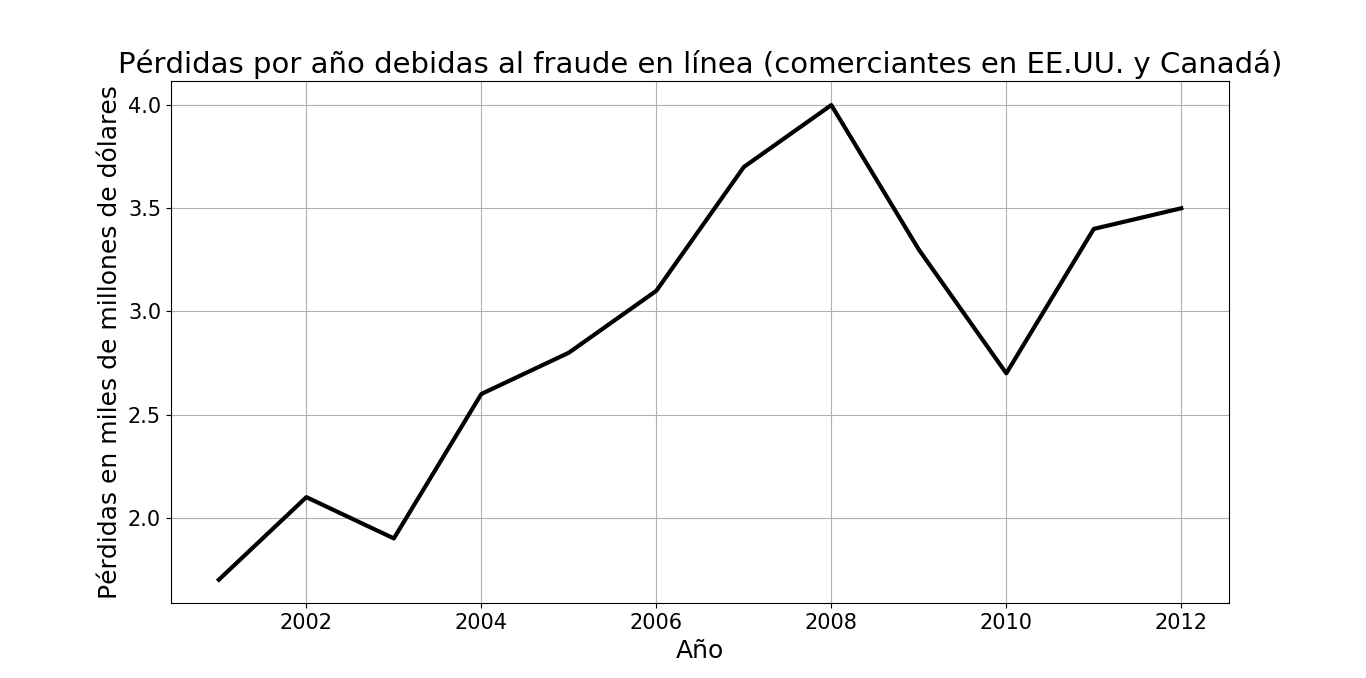
\includegraphics[width=0.85\linewidth]
       {diagramas_comunes/estadisticas_fraudes/perdidas_fraude_2002_2012.png}
    \caption{Pérdidas debidas al fraude en línea (2001-2012)~\cite{wallethub}.}
  \end{figure}
  \note{
    \begin{itemize}
      \item En la década de los 80 y 90 nadie previó el impacto que tendría el
        internet, no estaban preparados y mientras más se utilizaba el
        internet, más se acrecentaron los fraudes de tarjetas.
      \item Recalcar que las pérdidas mostradas en la gráfica son solo de
        fraudes en EE. UU. y Canadá.
    \end{itemize}
  }
\end{frame}

\begin{frame}{Planteamiento del problema}
  {La protección de datos bancarios}
  \begin{figure}
    \centering
    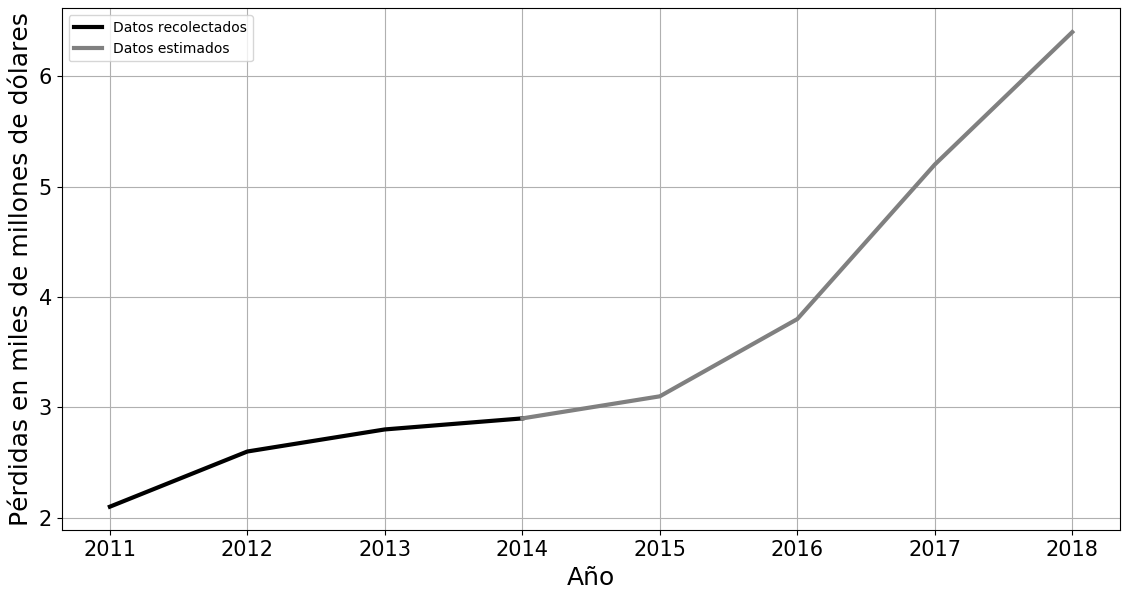
\includegraphics[width=1\linewidth]
       {diagramas_comunes/estadisticas_fraudes/perdidas_fraude_2011_2018.png}
    \caption{Pérdidas debidas al fraude con tarjetas no presentes (CNP) en
              EE.~UU. (2011-2018)~\cite{creditcards}.}
  \end{figure}
  \note{
    \begin{itemize}
      \item Recordar que, a partir del 2014, los datos son estimados.
      \item Parece que las cifras no coinciden con la gráfica pasada, pero es
        porque aquí solo se están considerando los fraudes debido a tarjetas
        no presentes (la gráfica anterior contaba las pérdidas por tarjetas
        robadas/clonadas).
      \item Se proyecta un repunte de las pérdidas debido al desarrollo de un
        cambio en los chips de las tarjetas que hacen más difíciles los fraudes
        por tarjetas presentes.
    \end{itemize}}
\end{frame}

\begin{frame}{Planteamiento del problema}
  {Publicaciones del PCI}
  \begin{itemize}
    \item<1-> En 2004, se publicó el PCI DSS\footnotemark \cite{pci_dss}.
      \note<1>{
        Remarcar que antes del estándar unificado, cada quién intentó sacar sus
        buenas prácticas, pero, pues si para una PyME estaba medio en chino
        satisfacer uno, ahora satisfacer 3 o 4, pues nein. Oh, también
        mencionar quiées componen el concilio: Mastercard, VISA,
        AmericanExpress, Discovery...
        También recordar que solo es (era) obligatorio cumplir con él cuando
        se realizan más de 20K transacciones al año. Y que es MUY difícil de
        satisfacer, pues aunque tiene menos de 15 requerimientos, los
        subrequerimientos y subsubrequerimientos complican todo. }
    \item<2-> Hasta este momento, el enfoque era proteger la información en
      donde sea que se encuentre.
      \note<2>{
        Dar el típico ejemplo de esto: había que proteger la información de
        un cliente en el depto. de ventas, entregas, usuarios, ect. y la
        comunicación entre todos estos canales. Luego mencionar que el
        paradigma cambia y ahora ponen TODA la información valiosa en un mismo
        lugar, así solo hay que proteger este lugar. Recordar que un adversario
        no puede hacer mucho si solo tiene los tokens.}
    \item<3-> En 2011, el PCI SSC\footnotemark{} publicó las primeras guías
      para los procesos de tokenización~\cite{pci_tokens}.
      \note<3>{
        Aunque indica lo que debe satisfacer el sistema tokenizador,
        no dice cómo generar los tokens.}
  \end{itemize}

  \addtocounter{footnote}{-2}
  \stepcounter{footnote}\footnotetext{
    \textit{Payment Card Industry, Data Security Standard}}
  \stepcounter{footnote}\footnotetext{
    \textit{Payment Card Industry, Security Standards Council}}
\end{frame}
